\section{Auswahl der Objektdetektoren}

Für das \textit{Smart Warehouse} Szenario soll eine Auswahl zwischen den vier Detektoren \textit{Faster R-CNN}, \textit{Mask R-CNN}, \textit{SSD} und \textit{YOLO} getroffen werden. Als Vergleichsbasis dienen die bereits veröffentlichten Benchmarkergebnisse. Zur Evaluation der Machbarkeitsstudie werden die zuvor eingeführten Bewertungskriterien auf die aus dieser Auswahl resultierenden Objektdetektoren angewendet.

\begin{figure}[ht]
	\begin{center}
		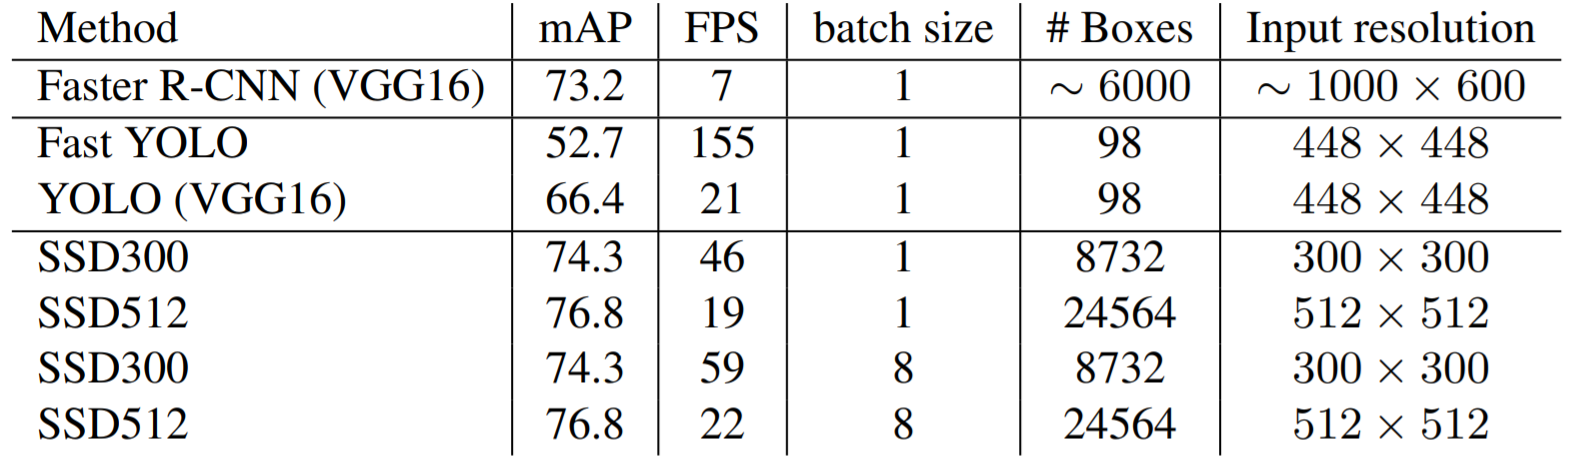
\includegraphics[width=12cm]{Bilder/ssd_results.png} 
		\caption[Vergleich SSD auf PascalVOC]{Vergleich SSD auf PascalVOC \cite{ssd.20161229}}
		\label{result}
	\end{center}
\end{figure}

Nach Tabelle \ref{result} ist eindeutig festzustellen, dass der \textit{SSD} bezüglich \textit{mAP} am besten abschneidet. \textit{Faster-RCNN} kann zwar bezüglich der \textit{mAP} mithalten, ist allerdings nicht zur schnellen Inferenz ausgelegt. \textit{YOLO} schneidet in beiden Kategorien schlechter als der \textit{SSD} ab. Dem \textit{SSD} gelingt es also, ein gutes Verhältnis zwischen Präzision und Reaktionsvermögen zu bewahren. Durch den Verzicht auf den Schritt der Generierung von Bounding Box Vorschlägen und des \textit{Poolings} kann \textit{SSD} deutlich schneller ablaufen als die Vergleichsdetektoren, während durch das Vordefinieren von Bounding Boxen ebenso eine hohe Präzision erzielt werden kann \cite{ssd.20161229}.

Allerdings ergibt sich vor allem für kleine Objekte ein erschwertes Detektionsvermögen, da diese in den höherliegenden Convolutional Layern untergehen. Als Lösung hierfür kann eine erhöhte Inputgröße gewählt werden (vgl. \textit{SSD512}) oder \textit{Data Augmentation} für den Lernprozess angewandt werden \cite{ssd.20161229}.

Diese Probleme treten bei Netzen der \textit{R-CNN} Familie nicht auf. Vergleicht man den \textit{Faster-RCNN} Objektdetektor mit \textit{Mask R-CNN} zur \textit{instanzbasierten Segmentierung} auf Basis des \textit{Common Objects in Context} (COCO) Datensatzes, so ergibt sich für \textit{Mask R-CNN} mit 38.2\% mAP nur eine geringe Verbesserung gegenüber \textit{Faster R-CNN} mit 37.3\%. Für diesen Benchmark wurde wohlbemerkt das \textit{RoI-Pooling Layer} des \textit{Faster R-CNN} mit einem \textit{RoI-Align Layer} zur besseren Vergleichbarkeit mit dem \textit{Mask R-CNN} Objektdetektor ausgetauscht. Dennoch bleibt auch beim \textit{Mask R-CNN} das Problem eines langsameren Inferenzverhaltens gegenüber dem \textit{SSD} oder \textit{YOLO} offen \cite{IntanPurnamasar.20181215}. 

Doch ist dieser Gesichtspunkt überhaupt relevant für das Einsatzszenario im \textit{Smart Warehouse}? Für einen generell industriellen Einsatz könnte dies wahrlich problematisch sein, doch für das konkrete Szenario von stehenden Getränkeflaschen in der Machbarkeitsstudie ist eine starke Gewichtung der FPS Metrik zunächst mit Vorsicht zu betrachten.

Ein weiteres Auswahlkriterium stellt dar, wie gut die Detektoren aufgesetzt und auf eigens erstellte Datensätze umkonfiguriert werden können. Nach Betrachtung mehrerer Repositories ließen sich der \textit{YOLO} und \textit{SSD} Objektdetektor einfach aufsetzen und auf eigene Datensätze anpassen, stellten bei \textit{Faster R-CNN} und \textit{Mask R-CNN} vermehrt auf Probleme gestoßen wurde. So ist Facebooks Implementierung von \textit{Mask R-CNN} \glqq Detectron\grqq{} beispielsweise nur auf Linux oder macOS lauffähig. Abgeleitete Repositories sind bereits als \textit{deprecated} deklariert und werden nicht mehr gewartet. Ein manuelles Aufsetzen dieser Implementierungen ist nur unter großem Aufwand möglich und wurde aufgrund der limitierten Zeit abgebrochen. Auch die Referenzimplementierung von \textit{Faster R-CNN} ist bereits als \textit{deprecated} deklariert und verweist auf die \textit{Mask R-CNN} Implementierung \textit{Detectron}. Nebenläufige Implementierungen sind ebenso als \textit{Legacy} Implementierungen vermerkt und nur zeitaufwändig manuell aufsetzbar, sofern sie die Windows-Plattform unterstützen.

Aufgrund dieser Umstände und des schlechteren Abschneidens in der zeitkritischen Modellinferenz wurden \textit{YOLO} und \textit{SSD} als die beiden Detektoren ausgewählt, die im \textit{Smart Warehouse} Szenario genutzt werden sollen. Für \textit{YOLO} wird die Referenzimplementierung im \textit{Darknet} Framework gewählt. Dieses lässt sich ebenso einfach auf eigene Datensätze anpassen im Gegensatz zur Referenzimplementierung des \textit{SSD} im \textit{Caffe} Framework. Deswegen wurde sich bei dem \textit{SSD} für eine Custom Implementierung in \textit{PyTorch} entschieden.






